%!TEX root = ../bare_jrnl.tex

\section{The Partially Observable Poisson Process}
\label{sec:popp}

The \emph{partially observable} Poisson process (POPP) is a counting process $N(t)$ with arrival rate $\lambda$ where the number of events appearing over the time interval $[0, t)$ are obtained by one or more \emph{unreliable} counters. 
% 
The definition brings a distinction between the \emph{true count} (or simply \emph{count}), which refers to the number of events that actually occurred, and the \emph{sensed count}, which refers to the count obtained by a counter (or sensor). Let $c_i$ represent the true count over the interval $[0, t)$ during the $i$-th observation. With $m$ counters unreliably observing $c_i$, we use  $s_{j,i}$ to represent the sensed count given by sensor $j$ in the $i$-th observation within the interval $[0, t)$ with $1 \leq j \leq m$. Let $\vec{s_i} = (s_{1,i}, \ldots, s_{m,i})$ represent a vector of sensed counts from $m$ sensors for the $i$-th observation of the process. 
% 

\begin{figure}[t!]
	\centering
	\begin{tikzpicture}
	\tikzstyle{place}=[circle,draw=blue,thick,minimum size=15 mm]
	\tikzstyle{small}=[circle,draw=blue,thick,minimum size=8 mm]
	\tikzstyle{every label}=[black]
	\begin{scope}
	\node[place](31)[xshift=0mm]{$\lambda$};
	\node[place](21)[below of=31, yshift=-10mm]{$C_i$} edge[pre](31);
	\node[small](11)[below of=21, yshift=-10mm]{$\ldots$} edge[pre](21);
	\node[place](12)[left of=11, xshift=-5mm]{$S_{2i}$} edge[pre](21);
	\node[place](13)[left of=12, xshift=-10mm]{$S_{1i}$} edge[pre](21);
	\node[place](14)[right of=11, xshift=5mm]{$S_{(m-1)i}$} edge[pre](21);
	\node[place](15)[right of=14, xshift=10mm]{$S_{mi}$} edge[pre](21);
	\draw[thick]($(13.north west)+(-0.5,2.45)$) rectangle ($(15.south east)+(0.5,-0.5)$);
	\end{scope}
	\end{tikzpicture}
	\caption{Graphical representation of the partially observable Poisson process.}
	\label{fig:gm_popp}
\end{figure}

%\begin{figure}[t!]
%	\centering
%	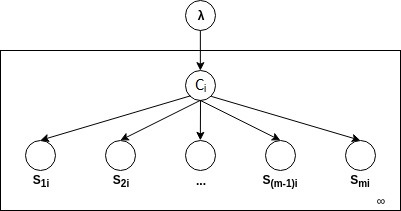
\includegraphics[width=0.5\textwidth]{./figures/gm_popp.jpg}
%    \caption{Graphical representation of the partially observable Poisson process.}
%	\label{fig:gm_popp}
%\end{figure}


Figure~\ref{fig:gm_popp} presents the graphical model derived from the definition of the POPP. This shows that the true count $c_i$ has become a latent variable which can only be inferred from the sensed count.
% 
The posterior of $\lambda$ is then inferred from the posterior of $c_i$ after $n$ observations, $i = 1 \ldots n$. 
% \textbf{TODO: Fix figure to have \emph{multiple} $c_i$s not a single $X_i$. \emph{$c_i$ can not be multiple since it is the true count at time interval $i$, the sensed count can be multiple since they may come from different sensors.}	}

The rate parameter $\lambda$ of the POPP model can be inferred by marginalising over all possible true count values $c_i$ in $P(\lambda ; c_i)$ and in the  distribution of true counts given sensed counts $P(c_i ; \vec{s_i})$. 
% 
Given $n$ observations of the underlying process, let all observed true counts be represented by $\vec{c} = (c_1, \ldots, c_n)$, and all sensed counts by $\vec{s}=(\vec{s_1} \dots \vec{s_n})$, for $1 \leq i \leq n$ (recalling each $\vec{s_n}$ is produced by $m$ sensors). 
% 
The posterior of $\lambda$ is then:
\begin{equation}
	\label{eq:marginal_occurrences}
	\begin{tabular}{r@{=}l}
		$P(\lambda ; \vec{s})$ &  $\displaystyle\sum_{c_1=0}^{\infty} \ldots \displaystyle\sum_{c_n=0}^{\infty} P(\lambda ; \vec{c}) ~ P(\vec{c} ; \vec{s})$ \\
	\end{tabular}
\end{equation}
\noindent where true count probabilities, $P(\lambda ; \vec{c})$, can be drawn from the original FOPP definition:
\begin{equation*}
	\begin{tabular}{r@{ = }l}
		$P(\lambda ; \vec{c})$ & $Gam\Bigg(\lambda ; \displaystyle\sum_{i=1}^{n} c_i + \alpha, n + \beta \Bigg)$
	\end{tabular}
\end{equation*}


If we assume that the sensor counts for observation period $i$ are conditionally independent (i.e.~\textit{uncorrelated}) given the true count $c_i$, then the probability of a collection of observations given the true count, can be defined as follows: 

\begin{equation}
	\label{eq:independent_sensor_likelihood}
	\begin{tabular}{r@{=}l}
	$P(\vec{s_i} ; c_i)$ & $\displaystyle\prod_{j=1}^{m} P(s_{j,i} ; c_i)$ \\ 
	\end{tabular}
\end{equation}

Using this, the probability of a particular sequence of $n$ counts, given a sequence of $n$ observations each from $m$ sensors, $P(\vec{c} ; \vec{s})$, can be defined as:

\begin{equation}
    \label{eq:occurrences_likelihood}
    \begin{tabular}{r@{ $\varpropto$ }l}
        $P(\vec{c} ; \vec{s})$ & $P(\vec{s_1}, \ldots, \vec{s_n} ; \vec{c}) ~ P(\vec{c})$ \\ [1ex]
        & $\displaystyle\prod_{i=1}^{n} P(\vec{s_i} ; c_i) ~ P(c_i)$ \\ [2ex]
        & $\displaystyle\prod_{i=1}^{n} \displaystyle\prod_{j=1}^{m} P(s_{j,i} ; c_i) ~ P(c_i ; \vec{c_{-1}})$
    \end{tabular}
\end{equation}

\noindent where $\vec{c_{-1}} = c_{i-1}, \ldots, c_1$, and $P(c_i ; \vec{c_{-1}})$ can be calculated using a negative binomial distribution:

\begin{equation}
	\label{eq:unconditional_xi}
	\begin{tabular}{r@{=}l}
		$P(c_i ; \vec{c_{-1}})$ & $\displaystyle\int_{\lambda=0}^{\infty} P(c_i ; \lambda) ~ P(\lambda ; \vec{c_{-1}}) ~d\lambda$ \\ [2ex]
		& $\displaystyle\int_{\lambda=0}^{\infty} Poi(c_i ; \lambda) ~ Gam(\lambda ; \alpha, \beta) ~d\lambda$ \\ [2ex]
		& $NB\Bigg(c_i ; \alpha, \displaystyle\frac{\beta}{\beta + 1}\Bigg)$.
	\end{tabular}
\end{equation}

To complete Eqn. \ref{eq:occurrences_likelihood} we must also define $P(s_{j,i} ; c_i)$. The Poisson limit theorem states that the Poisson distribution may be used as an approximation to the binomial distribution \cite{papoulis2002probability}. Using this theorem as the foundation, an arbitrarily close approximation to the probability $P(s_{j,i} ; c_i)$ is defined by assuming there exists a small enough finite subinterval of length $\delta$ for which the probability of more than one event occurring is less than some small value $ \epsilon$. With this assumption, interval $[0, t)$ is split into $l$ smaller subintervals $I_1, \ldots, I_l$ of equal size, with the condition that $l > \lambda$. Consequently, the whole interval $[0, t) = I_1, \ldots, I_l$ becomes a series of Bernoulli trials, where the $k^{th}$ trial corresponds to whether (1) an event $e_k$ happens with probability $\lambda / l$ and (2) a sensor $j$ captures the event $e_k$ as the detection $d_k$ at the subinterval $I_k$.

Following this, $P(s_{j,i} ; c_i)$ can be defined using of the count of true  positives over $c_i$ subintervals, and false positives over the remaining $l-c_i$ subintervals. 
% 
Let the probability of a \textit{true positive detection} (TP) for sensor $j$ in a single subinterval be $\tau_j = P_j(d;e=1)$, and the probability of a \textit{false positive detection} (FP) be $\xi_j = P_j(d;e=0)$. Thus $P(s_{j,i} ; c_i)$ is defined as a sum over all possible sensed counts of the product of two binomial distributions $B(r ; n,\pi)$: 

\begin{equation}
	\label{eq:joint_binomial_distribution}
    P(s_{j,i} ; c_i) \! = \! \! \! \displaystyle\sum_{r = 0}^{c_{i}} \! \! B\Big(r ; c_i, \tau_j\Big) B\Big((s_{j,i} - r) ; (l - c_{i}), \xi_j \Big)
\end{equation}
\noindent where the first binomial provides the probability of getting some proportion of the count from  TP detections and the second binomial provides the probability of getting the remainder from FP detections. 

% \textbf{NOTE: This constraints $s_{j,i} \leq c_i$, doesn't it? Is it worth commenting on this? If we don't want this then we need to introduce $l$ a little more formally than was done before. \emph{we do not constraint it, $s_{j, i}$ can be greater than $c_i$. if $s_{j, i}$ is greater than $c_i$ it means that some portion of $s_{j, i}$ contains false positive.}}

Eqn.~\ref{eq:marginal_occurrences} shows the difficulty of estimation in the POPP model. Since no conjugate density provides an analytical solution for the posterior over $\lambda$, every sensed count $\vec{s_i}$ must be retained to calculate the posterior of $\lambda$. Therefore each of the $n$ observation periods adds a factor of a countably infinite number of elements, and therefore the posterior is a sum of countably infinite sums. Even with an upper bound $l$ on the maximum value of $c_i$, the number of elements in the posterior grows by $l$ with each observation period.
% 
\subsection*{$\lambda$ Estimators}

With this difficulty noted, we previously proposed three efficient estimators, each of which offers an approximation to the true posterior $P(\lambda ; \vec{s})$. Three efficient estimators we proposed in \cite{jovan18a} are: \\
(1) \textit{Gamma filter}, which approximates Eqn.~\ref{eq:marginal_occurrences} with a single gamma minimising the KL-divergence $D_{KL}(P(\lambda ; \vec{s}) \mid \mid Gam(\lambda \mid \alpha, \beta))$ by gradient descent. This filter gradually worsens as sensor reliability degrades; \\
(2) \textit{Histogram filter}, which approximates Eqn.~\ref{eq:marginal_occurrences} with a discrete distribution $Q(\lambda ; \vec{s})$ by quantising $\lambda$ to discrete values. The advantage of this filter over the gamma filter is that it can track the posterior to an arbitrary fidelity via finer quantisation. The disadvantage is increased computational time by at least ten fold compared to the gamma filter; \\
(3) \textit{Switching filter}, which approximates Eqn.~\ref{eq:marginal_occurrences} either by a gamma filter or by a histogram filter depending on whether $P(\lambda ; \vec{s})$  resembles a gamma distribution and can be approximated by the gamma filter via KL-divergence $D_{KL}(P(\lambda ; \vec{s}) \mid \mid Gam(\lambda \mid \alpha, \beta))$.

\begin{figure}[t!]
	\centering
	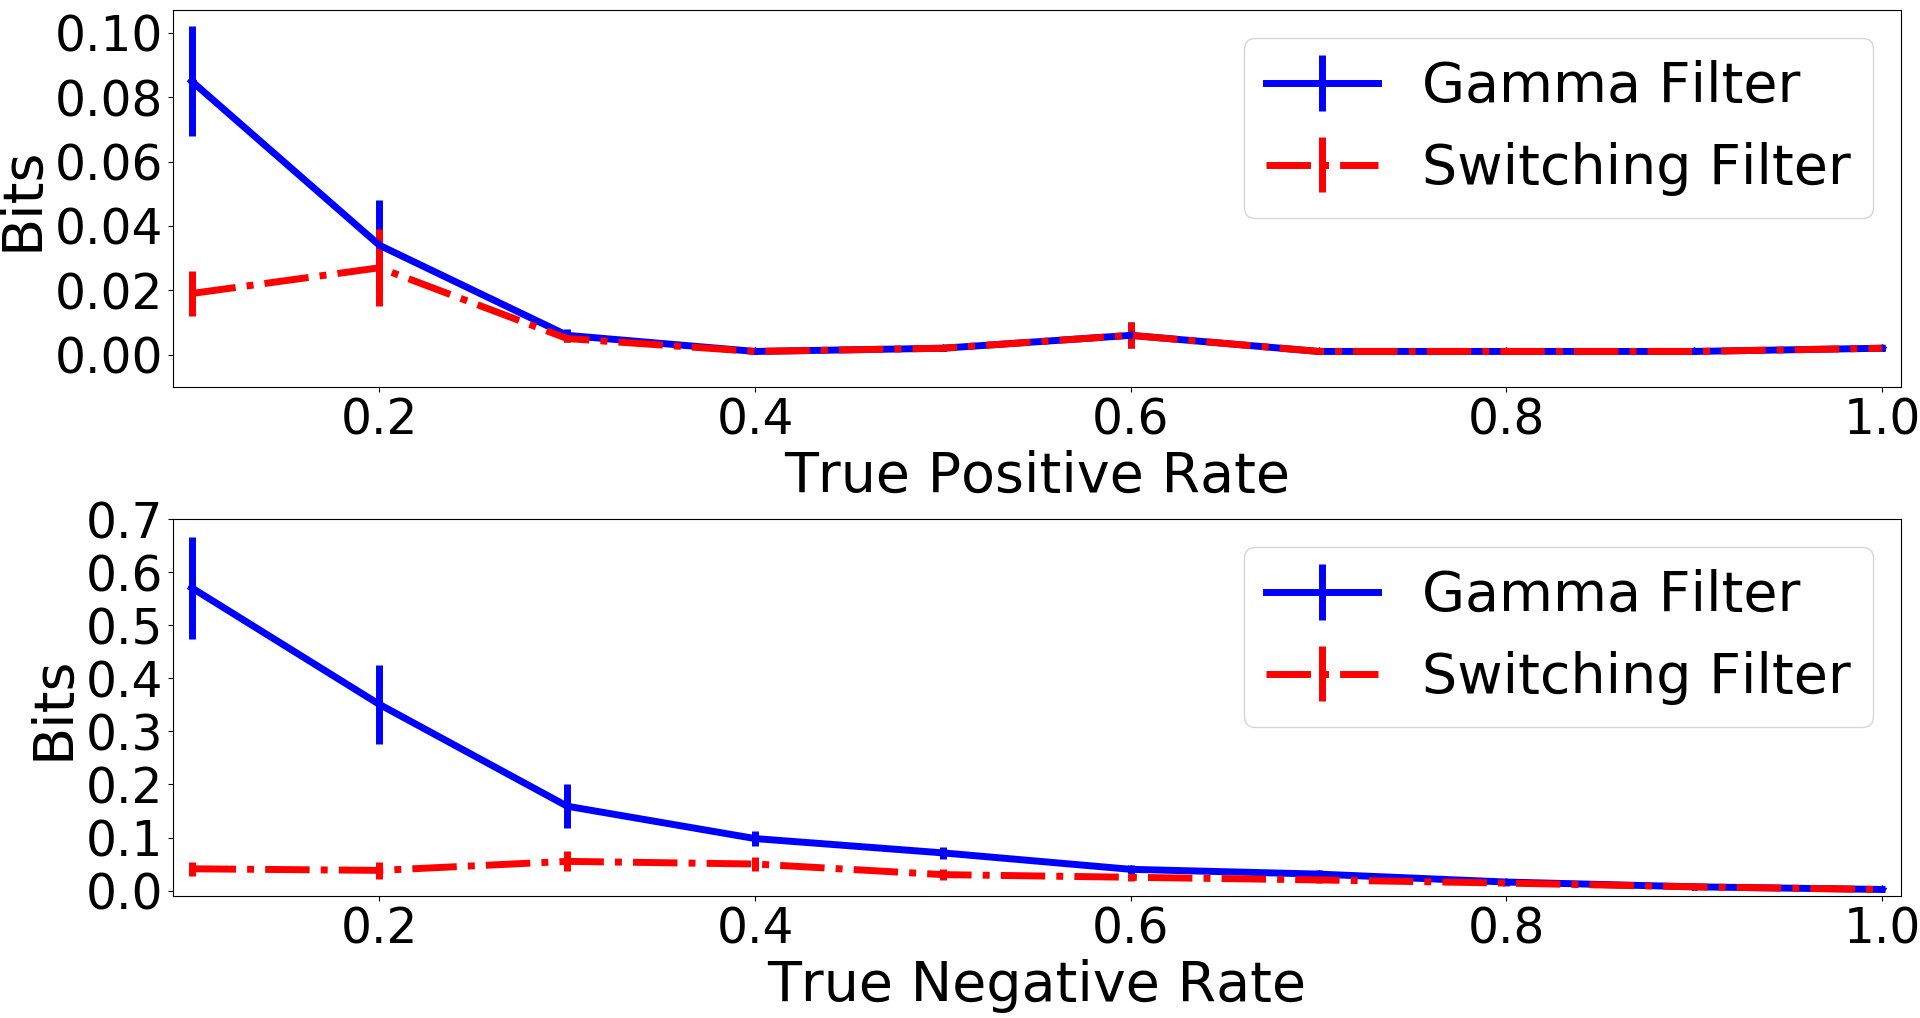
\includegraphics[width=0.5\textwidth]{./figures/kl_div_tpr_tnr_var.png}
	\caption{Average KL-divergence from the gamma and switching filters to $P(\lambda \mid \protect\vec{s})$. The horizontal axis shows the true positive rate (top) and true negative rate (bottom) of one simulated sensor. Standard error is shown. \cite{jovan18a}} 
	\label{fig:kl_div_tpr_tnr_var}
\end{figure}

Following \cite{jovan18a}, we propose the use of switching filter as the estimator to the true posterior $P(\lambda ; \vec{s})$ because the switching filter takes the best of both the gamma filter (fast calculation) and the histogram filter (accurate approximation) with minimum loss in similarity to the true posterior $P(\lambda ; \vec{s})$. Figure \ref{fig:kl_div_tpr_tnr_var} showed how (dis)similar both the gamma filter and the switching filter to the true posterior in terms of the KL-divergence on different sensor reliability using simulated data. Note that the histogram filter was not included because it perfectly tracked $P(\lambda ; \vec{s})$, i.e., $D_{KL}(P(\lambda ; \vec{s}) \mid \mid Q(\lambda ; \vec{s})) \approx 0$. A more detailed presentation of these estimators is given in \cite{jovan18a}.